
\documentclass{article}
\usepackage{amsmath}
\usepackage[utf8]{inputenc}
\usepackage{subfig}
\usepackage{graphicx}

\usepackage{amsbsy}
\usepackage{hyperref}
%\title{Deep Reinforcement Learning for Perspective Taking Task}
\title{Perspective-Taking Using Deep Reinforcement Learning}
\author{Aqeel Labash}
\date{September 2017} 
\usepackage{natbib}
\usepackage{graphicx}
\usepackage{makecell}
\usepackage{float}
\begin{document}
\maketitle
\section{Abstract}
Perspective taking is the ability take the point of view of another agent. This capability is not unique to humans but extends to other organisms like chimpanzees\cite{hare2000chimpanzees}. It is an essential ability to achieve efficient social interactions, including cooperation and competition. In this work, we present our progress toward reverse engineering how perspective taking task might be accomplished in our brains. We created perspective-taking tasks, in which the environment is partially observable by its agents. We also show a model that was able to pass multiple tests that would benefit from perspective taking capabilities. The model was trained using reinforcement learning algorithms assisted by artificial neural networks.

\section{Introduction}
When two persons are in a room that is familiar to both of them, they do not need to switch places to imagine what another can see and cannot see. Looking at things from a perspective that differs from our own is called perspective taking \cite{ryskin2015perspective}. It could be defined as "the cognitive capacity to consider the world from another individual's viewpoint" \cite{davis1983measuring}. According to Galinsky and colleagues, it is one of the social competencies that motivates social understanding in many contexts \cite{galinsky2008pays}.

Many decisions we take depend on others, what they think, what they believe, and what we know about what they know. This ability to understand and infer the mental states of others is called \textit{theory of mind} \cite{premack1978does} or mindreading \cite{apperly2011mindreaders}. Somewhat surprisingly not only humans have the ability to take into consideration what others think and believe. In controlled experiments, it has been shown that chimpanzees can know what other chimpanzees see and know \cite{hare2000chimpanzees}. Here we ask whether artificial intelligence (AI) agents using neural networks could also learn to infer what other agents perceive and know. In particular, we test here the ability of reinforcement learning agents to learn one essential part of \textit{theory of mind}: perspective taking. 

\par Perspective taking ability is not unique to humans but extends to chimpanzees \cite{hare2000chimpanzees}. Chimpanzee social status is organized hierarchically (dominant, subordinate) \cite{goldberg1997genetic}. When there is food available that both can reach, the dominant always gets it. In the experiments \cite{hare2000chimpanzees}  two chimpanzees were set into two separate cages facing the other with food positioned between them as shown in Figure \ref{tom.experiment} (left). The three conditions differed mainly in what the dominant and the subordinate can see. For example in the "subordinate door" condition one piece of food cannot be seen by the dominant chimpanzee. Can the subordinate take advantage of this fact? The results are shown in Figure \ref{tom.experiment} (right) and demonstrated that the subordinate indeed obtained more food in this condition. Hence, the subordinate was able to take into account what the dominant chimpanzee could see. In other words, the subordinate could take the perspective of the dominant chimpanzee. For other experiments and details see for example \cite{hare2000chimpanzees, de2016we, tomasello2009cultural}.  

\begin{figure}[!ht]
\begin{center}
\includegraphics[scale=0.3]{figures/tom_experiment_1.png}
\includegraphics[scale=0.3]{figures/tom_experiment_1_results.png}
\caption{Left: three different positions for the food with different ability to observe it (food indicated by black ellipses, cage walls indicated by lines). Right top: Average percentage of eaten food by subordinate between different food positions. Right bottom: the average percentage based on food visibility condition. \cite{hare2000chimpanzees}}
\label{tom.experiment}
\end{center}
\end{figure}

We designed an environment \texttt{APES} that allowed us to simulate experiments in \cite{hare2000chimpanzees} where a subordinate chimpanzee chose whether to go for food or not depending on the observability of the food by the dominant chimpanzee. The aim of the present work is to study whether an AI agent controlled by a neural network can learn to solve similar perspective taking task using reinforcement learning (RL).

RL is a branch of AI that allows an agent to learn by trial and error while interacting with the environment. In particular, the agent must learn to select the best action in each specific state to maximize its cumulative reward \cite{sutton1998reinforcement}. The agent could be an autonomous robot \cite{lin1993reinforcement,yang2004multiagent,riedmiller2009reinforcement} or a character in video game \cite{mnih2013playing,tampuu2017multiagent} or even computer simulations based of biological systems \cite{amigoni2007multiagent}. 

\par 
The idea behind learning by interacting with an environment is inspired from how human and animal infants learn from the rich cause-effect or action-consequence structure of the world \cite{sutton1998reinforcement,thorndike1911animal,schultz1997neural}. Therefore, RL is a biologically plausible method of learning certain associations and behavior. 

We do not think that RL captures all aspects of perspective taking or is the exact model how perspective taking is learned in biological organisms (Aru \& Vicente, submitted). However, we hope that understanding the capabilities and limitations of RL in acquiring perspective taking skills will lead to a better algorithmic understanding of perspective taking in biological organisms.
\section{Background}

\subsubsection{Deep Q-Networks} \label{Deep.Q.L}
Deep Q-Networks (DQN) is the result of combining deep learning with Q-learning \cite{watkins1989learning,watkins1992q} algorithm which is one of the most important algorithms in RL \cite{sutton1998reinforcement}. The idea is to use neural networks to approximate the Q-value function. The algorithm proceeds by saving transitions (state \(s_t\), action \(a_t\), reward \(r_t\), and the new state \(s_{t+1}\)) to be used later to train a network parametrized by a vector \(\theta\). \cite{mnih2015human} used two networks (a training network parametrized by \(\theta\) and a target network parametrized by \(\theta^{-}\) which is updated at every time step according to (\(\theta^{-} = \theta \times \tau + \theta^{-} \times (1-\tau)\)). In this case the cost function to be minimized by the training network is the distance between its prediction and the following target value:

\begin{equation} \label{eq:0.06}
    y_t=
    \begin{cases}
      r_t, & \text{if its terminal state} \\
      r_t+ \lambda \underset{a'}{\max}Q(s_{t+1},a';\theta^{-}) , & \text{otherwise}  \, .
    \end{cases}
\end{equation}
\section{Methods}
To train a model capable of solving tasks that require perspective taking, three ingredients were needed. First, an environment to simulate the task. Second, a neural network model. Third, a training strategy for acquiring perspective taking since its not a straightforward task to be learned end to end.
%=============================================
\subsection{Environment}
%\textbf{General speaking about the envrionment functionality like you can use 10 agents etc .. }
\textit{APES} contains features like multi-agents possibility, partial observability and binary environment representation \cite{APES}. Figure \ref{fig.env} shows an example of the environment. \textit{APES} has 4 basic structures
\begin{enumerate}
    \item \textbf{World}:The arena where all elements are located.
    \item \textbf{Agent}:The most interactive element in the environment. After each step, each agent gets a reward and its perspective view of the world. Agent turn is to pick an action depending on the feedback received from the environment. The agent has many options depending on the required need. Following is an explanation of those features.
    \item \textbf{Obstacle}:Responsible for stopping agent from moving freely in the world. Obstacle element have the following features:
    \item \textbf{Food}:Main source for the positive reward\footnote{although it is possible to assign negative energy to represent poisoned food.}.
\end{enumerate}
The number of different objects( agents,obstacles,foods) is limited only by the world size.For more details the reader can access the \href{https://github.com/aqeel13932/APES}{github repository}
\begin{figure}[!ht]
\begin{center}
\includegraphics[scale=0.25,trim={3.2cm 3cm 2cm 3cm},clip]{figures/full_map.jpg}
\caption{Example image of the environment} \label{fig.env}
\end{center}
\end{figure}

%==============================================================
\subsection{Model}
We kept the model simple and straight forward. We used a feedforward neural network \cite{Goodfellow-et-al-2016}. Our model estimate state value, and advantages which is similar to dueling network \cite{DBLP:journals/corr/WangFL15} but instead of splitting the last layer we used all of it for value and advantages. Figure \ref{fig.model} shows our model. In our task no convolutional neural networks were used. Each experiment generated two models: 1) training model, which is updated every time step, 2) target model which $\tau$-averaged copy of training model weights every step.
  \begin{equation} \label{eq:model.mod}
    Q(s,a;\theta,\alpha,\beta) = V(s;\theta,\beta) +\left( A(s,a;\theta,\alpha) - \underset{a' \in |A|}{\max}A(s,a';\theta,\alpha) \right)
  \end{equation}
\par For training neural networks we used \texttt{Keras} library \cite{chollet2015keras}.
\begin{figure}[!ht]
\begin{center}
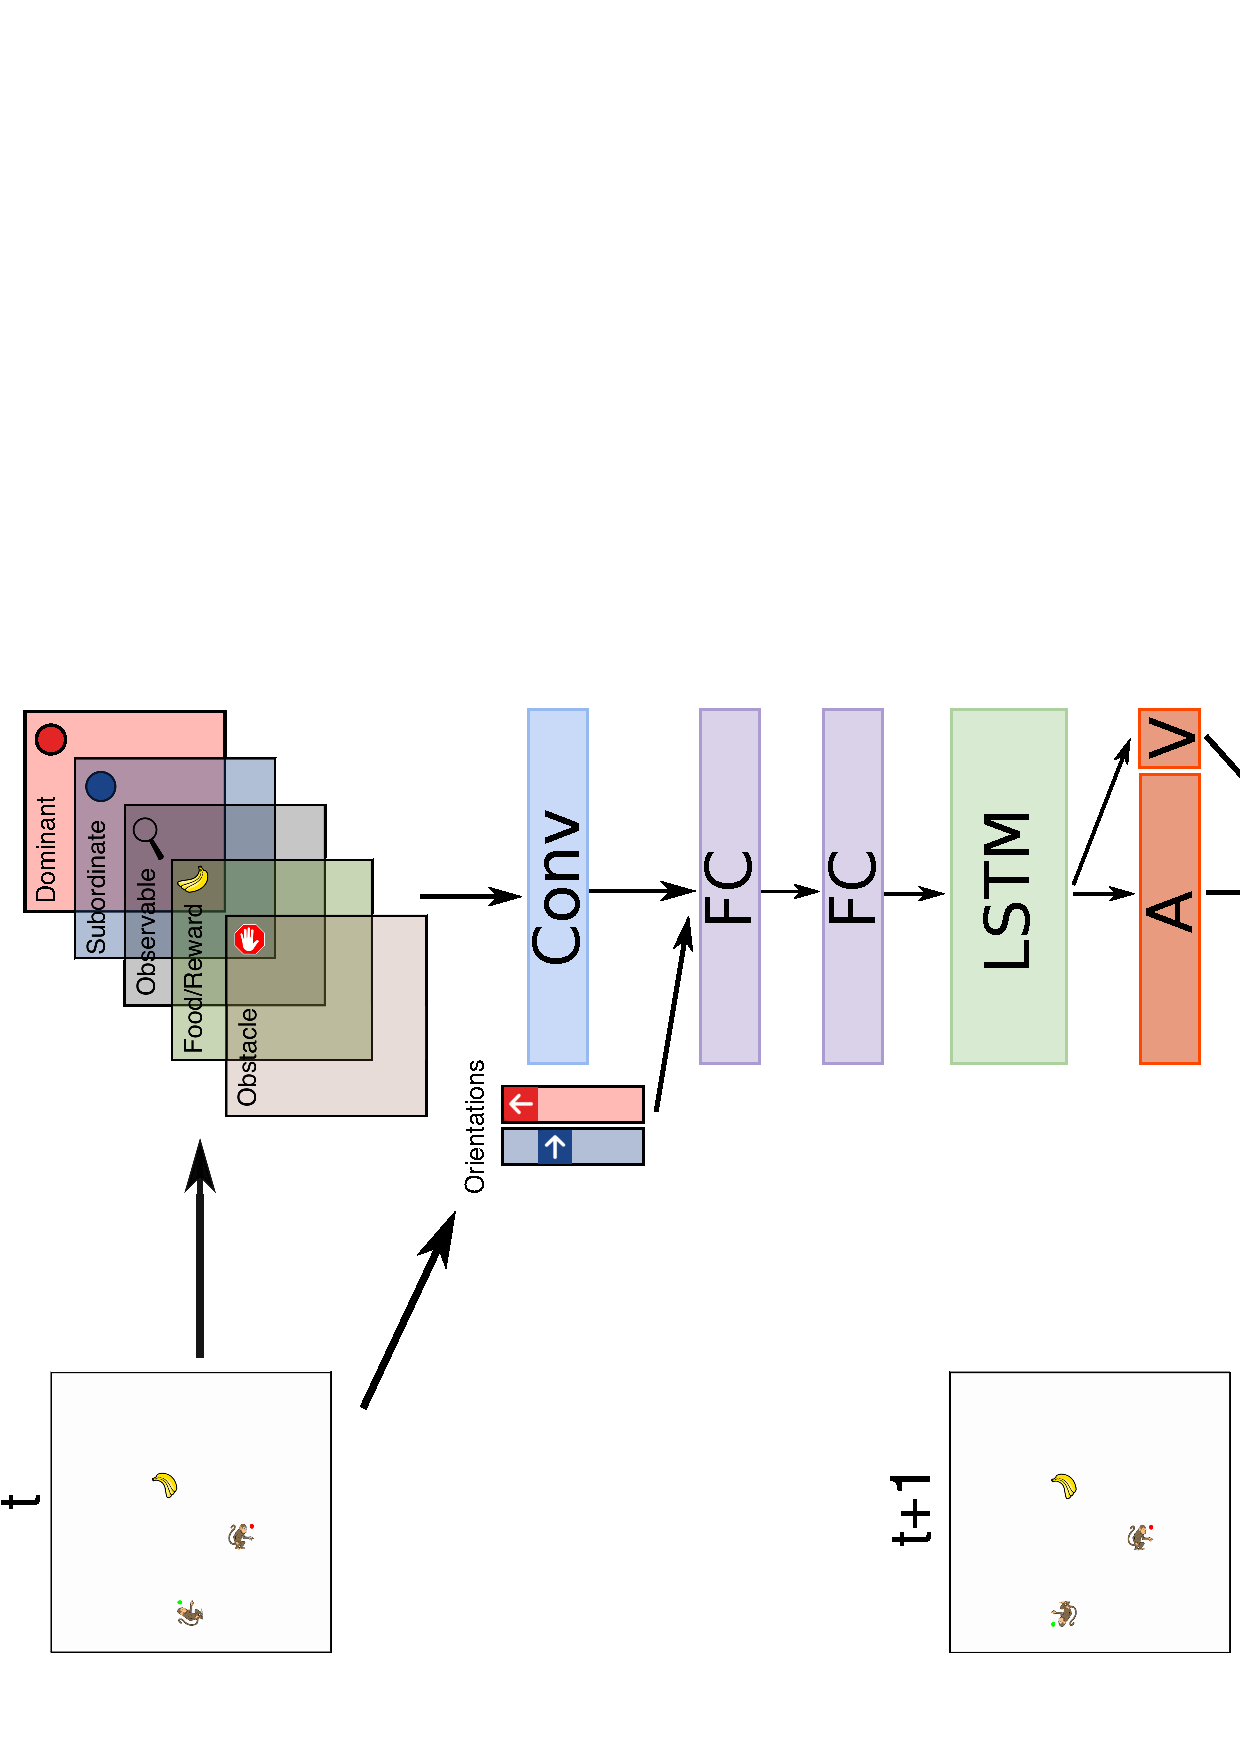
\includegraphics[scale=0.5]{figures/model.png}
\caption{Feedforward network where the connections between the last layer and the Q-values is regulated by formula \ref{eq:model.mod}}
\label{fig.model}
\end{center}
\end{figure}

\subsubsection{Network Input}
Information accessible to the agent from its visual field was fed as input to the agent's network in the form of binary feature vectors. Separate binary map was used for agent position, dominant agent position, food position, observed area and obstacles position. In addition one-hot vector of size 4 for each agent was added to represent agent's direction.
\subsubsection{Replay Memory}
Replay memory is a common practice when deep learning is used for RL tasks\cite{DBLP:journals/corr/WangFL15,mnih2015human,mnih2013playing}.
Reply memory helps to uncorelate the experiences for learning hence stabilizing learning. It also mimics a primitive model of hippocampus.
The replay memory or experience replay is a set of transitions (\(s_t,r_t,a_t,s_{t+1},terminal\)) which is used to train the network.  \par Each time step we trained the network with 32 randomly selected samples from the replay memory. We used a replay memory of size 100K. Once the replay memory is full oldest samples would be replaced.
\subsection{Perspective-taking Task}
The task we used included two agents: dominant $A_{dom}$ and subordinate $A_{sub}$. $A_{dom}$ and $A_{sub}$ are placed in an arena that contain obstacles $O$ that block vision and food $F$ which is the reward. The $A_{sub}$  need to get the food while keeping certain distance from dominant, otherwise it will be punished. $A_{dom}$ is driven by deterministic algorithm to find the food.
\subsection{Curriculum learning}
Curriculum learning consist of training an agent on a sequence of tasks of increased complexity to improve the speed of learning in a more complex task \cite{narvekar2016curriculum}. We defined tw tasks explained in the following sections where trained the agent first to find the food (Task 1) after that to avoid the dominant (Task 2).
\subsubsection{Task 1: finding the food} \label{task1}
In this stage the only task \(A_{sub}\) had was to find the food and eat it. This task might look easy but when we consider the vision and the obstacles it gets more complicated. Without a memory the agent has to act depending on the immediate vision of field. This stage optimized \(A_{sub}\) to look for the food and approach it. To make the task reasonable the obstacle will spawn randomly in specific region as shown in Figure \ref{fig:probabilities}. In this stage the input representing dominant agent is zeros.

\subsubsection{Task 2: avoiding dominant agent}\label{task2}
Finally, we trained the subordinate agent with a punishing dominant agent. The dominant gave -100 reward points for the subordinate whenever the subordinate was 1 or 2 steps away \footnote{both experiments were conducted separately.} from the dominant. 

\subsubsection{Reward scheme \label{reward.scheme}}
We used a reward scheme to grossly mimic some of the incentives found in the situations we are aiming to model. The agent has three types of reward,
\begin{itemize}
\item First, the agent receives a -0.1 per time step regardless of the chosen action to encourage finishing the task as soon as possible.
\item Second, the agent receives a reward of value 1000 for consuming food.
\item Third, the $A_{sub}$ gets a punishment of -100 each time enter the $A_{dom}$ control range.
\end{itemize}  
\subsection{Behavioral test cases}\label{agents.behavior}
We created 10 behavioral tests cases where none of them can be accomplished without perspective taking. In those test cases we tried to cover all the possible factors. Mainly we stabilized all elements (dominant, subordinate, food, obstacle) positions with exception of one of them at a time.
In addition to different types we tried 5 variation of each test case to make sure that results weren't just a statistically calculated. The test cases can be found 

\begin{itemize}

\item \textbf {Test case 1:} in this test the subordinate agent \(A_{sub}\) optimally supposed to go for the food since the food is unobserved by the dominant agent \(A_{dom}\). At the same time \(A_{sub}\) cannot see \(A_{dom}\). Environment in Figure \ref{fig.test.1.2.3} (a,b,c)

\item \textbf {Test case 2:} the target behavior from \(A_{sub}\) is to avoid the food as the dominant agent \(A_{dom}\) is visible and can see the food. Environment in Figure \ref{fig.test.1.2.3} (d,e,f)

\item \textbf {Test case 3:} \(A_{sub}\) supposed to go for the food in case \(A_{dom}\) was not spotted in its field of vision before eating the food. Environment in Figure \ref{fig.test.1.2.3} (g,h,i)

\item \textbf {Test case 4:} \(A_{sub}\) and \(A_{dom}\) can see each other while only \(A_{sub}\) can see the food. \(A_{sub}\) supposed to go for the food since the dominant does not see the food. Environment in Figure \ref{fig.test.4.5.6} (a,b,c)

\item \textbf {Test case 5:} only \(A_{dom}\) can see the food and both agents cannot see each other. \(A_{sub}\) is not supposed to go for the food as it cannot see the food and the food is under the dominant watch. Environment in Figure \ref{fig.test.4.5.6} (d,e,f)

\item \textbf {Test case 6:} agents can see the food but not each other. \(A_{sub}\) should go to food as long as \(A_{dom}\) is not spotted before taking the last action. Environment in Figure \ref{fig.test.4.5.6} (g,h,i)

\item \textbf {Test case 8:} agents can see each other but only \(A_{sub}\) can see the food. Similar case to Figure \ref{fig.test.4.5.6} (a,b,c) but \(A_{dom}\) here is closer to food. The expected behavior is to go for the food. Environment in Figure \ref{fig.test.7.8.9} (d,e,f).
\item \textbf {Test case 9:} \(A_{sub}\) can see both food and \(A_{dom}\) while the latter cannot see neither \(A_{sub}\) nor the food. \(A_{sub}\) supposed to go for the food as the dominant is looking away. Environment in Figure \ref{fig.test.7.8.9} (g,h,i).
\ref{fig.test.7.8.9} (a,b,c).

\item \textbf {Test case 10:} \(A_{sub}\) see all other elements while \(A_{dom}\) does not.\(A_{sub}\) supposed to go for the food. Environment in Figure \ref{fig.test.10.11.12} (a,b,c)

\item \textbf {Test  case 16:} \(A_{sub}\) and \(A_{dom}\) can see the food, but can not see each other.
\end{itemize}
\subsection{Experiments}
We created a $11\times11$ grid world environment. The elements in the environments have certain places to spawn in every episode with Driclicht distribution. Figure\ref{fig:probabilities} show the elements possible locations at the beginning of every episode. 
\begin{figure}[H]
    \centering
    \includegraphics[scale=0.5,trim={0cm 1cm 0cm 0cm},clip]{figures/probabilities.png}
    \caption{Show the possible start position for each element in the environment. Agent 1: is the subordinate, Agent 2 is the dominant.(Best seen with colores)}
    \label{fig:probabilities}
\end{figure}
\subsection{Hyper-parameters tuning}
During the tuning we explored many values for parameters in Table \ref{tab:best.hyp}. Typically we ran grid search procedure for different combinations of pairs of parameters.
\par Choosing the best hyper-parameters was based on the training average reward over multiple random seeds. Table \ref{tab:best.hyp}  show the best hyper-parameters that fit our task.

\begin{table}[H]
    \centering
    \begin{tabular}{*{2}{|c|}}
    \hline
         \textbf{Replay memory}& 100K\\
         \hline
         \textbf {\# layers }&1\\
         \hline
         \textbf {Hidden nodes}&100\\
         \hline
         \(\boldsymbol{\tau}\)&0.001\\
         \hline
         \textbf {Advantage}&\texttt{max} \\
         \hline
         \textbf {Activation}&\texttt{tanh}\\
         \hline
         \(\boldsymbol{\epsilon}(exploration)\)&0.01\\
         \hline
         \textbf {Batch size}&32\\
         \hline
         \textbf {Training repeat} &1\\
    \hline
    \end{tabular}
    \caption{best hyper-parameters}
    \label{tab:best.hyp}
\end{table}

Those hyper-parameters performed the best over multiple random seeds. We used them for the rest of the experiments.

\subsection{Training}
We trained our models on curriculum learning. First we trained it on task 1 for 2 million steps and exploration 1 which decrease to reach 0.1 after 1,5 million steps. Afterward we trained the model on task 2 for 500k step with exploration 0.1 from the beginning. During both tasks the subordinate agent got punished with -0.1 regardless if the agent move or not and 1000 for eating the food. In task 2 we added punishment of -100 for every time step the subordinate located next to dominant position and in its vision. While training dominant agent always move in random steps toward unexplored area. Once the dominant spot the food (reward) it move toward it immediately.

\section{Results}

\subsection{Behavioral test cases}
Our goal is to study whether deep RL agents could learn to infer what other agents can and cannot perceive. We tested our agents with 10 test cases designed to be accomplished only with perspective taking abilities. In those test cases we paused the dominant movement completely to see the emerged behavior from the subordinate. The following figures illustrate the test cases and the agent's behavior. The legend of each figure explains the situation and the behavior in more detail.

Our subordinate agent solved most of these test cases successfully demonstrating a capability for perspective taking. To control for the robustness of the results we included 4 sets of variations to the test cases where we shifted one or many elements by a pixel: 1- Shift all elements, 2- Shift dominant, 3- Shift Subordinate only, 4- Shift food position. In all these variations we observed similar results to the main results, hence confirming that our agent is not fooled by small variations of the data.

In table \ref{table:Tests} we summarize the results and show the expected behavior compared to the model behavior.
\begin{table}[H]
    \centering
    \begin{tabular}{|{c}||*{10}{c|}}
    \hline
    Test case&1&2&3&4&8&5&6&9&10&16\\
    \hline
    Video link&1&2&3&4&8&5&6&9&10&16\\
    \hline
    Figure&1&2&3&4&8&5&6&9&10&16\\
    \hline    
     \makecell{Dominant position \\ Food and obstacle  position}&DP&DP&DP&DP&DP&FO&FO&FO&FO&FO\\
    \hline
    \makecell{Expected behavior:\\Go or No}&Go&No&Go&Go&Go&No&No&Go&Go&Go\\
    \hline
    Actual behavior&Go&No&Go&Go&Go&No&No&Go&Go&Go\\
    \hline
    \end{tabular}
    \caption{show the test cases types and the expected behavior from the subordinate in each one. Last row show the actual behavior performed by the model.}
    \label{table:Tests}
\end{table}
\subsection{Testing the agent's behavior in perspective taking tasks}

\begin{figure}
    \centering
    \subfloat[]{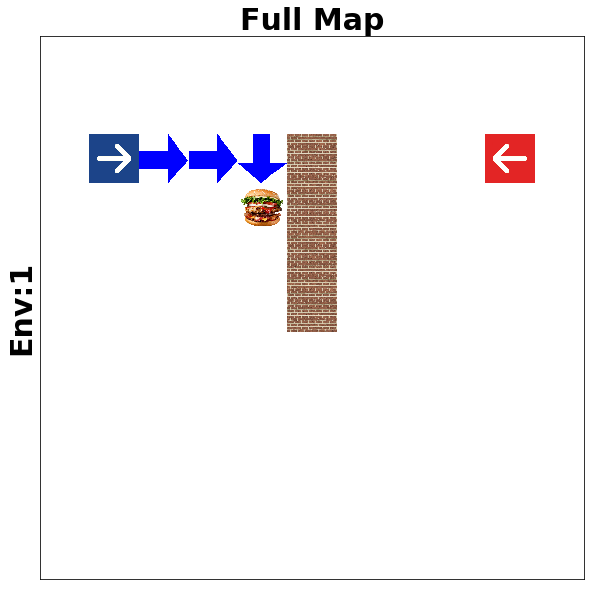
\includegraphics[scale=0.20]{figures/ENV:1_FM.png}}
    \subfloat[]{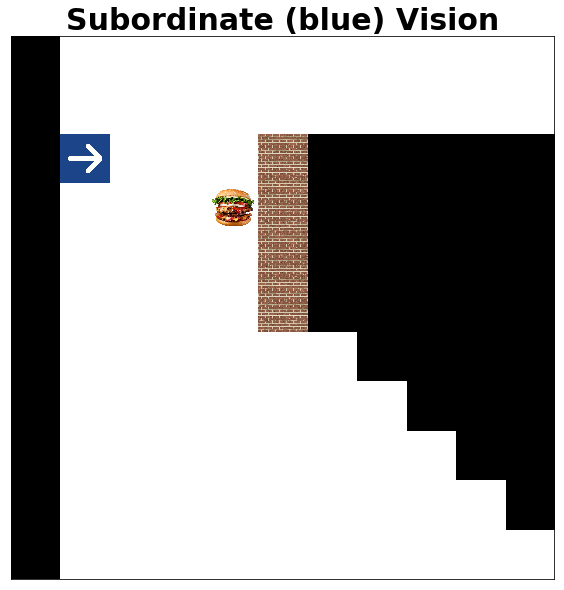
\includegraphics[scale=0.20]{figures/ENV:1_AI.png}}
    \subfloat[]{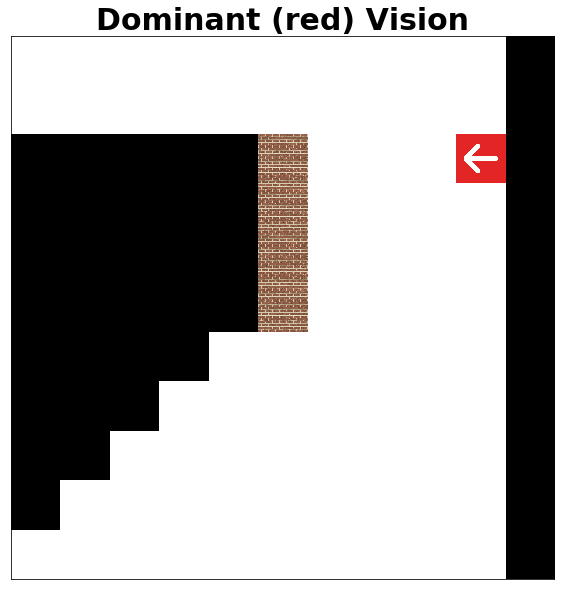
\includegraphics[scale=0.20]{figures/ENV:1_DM.png}}
    \caption{\textbf {Test  case 1:} \(A_{sub}\) did not see the dominant as the dominant was behind the obstacle. The subordinate \(A_{sub}\) went for the food in 6 steps. The followed path was optimal.  For this test case the agent achieved the expected behavior.}
    \label{fig.tc.1}
\end{figure}
\begin{itemize}
    \item \textbf {Test  case 1:} \(A_{sub}\) did not see the dominant as the dominant was behind the obstacle. The subordinate \(A_{sub}\) went for the food in 6 steps. The followed path was optimal.  For this test case the agent achieved the expected behavior.
    \item \textbf {Test  case 2:} \(A_{sub}\) avoided the food although the food is in the same position as in \texttt{Test case 1}. The only difference is the dominant position and direction: the dominant can see the food. The observed behavior is also what one would expect from an agent with the perspective taking ability.
    \item \textbf {Test  case 3:} \(A_{sub}\) went for the food, although the dominant is there and able to see everything. However, the dominant was out of the field of vision of the subordinate and hence the subordinate never witnessed \(A_{dom}\) until the very last move of eating the food. This behavior is also expected to happen.
    \item \textbf {Test  case 4:} in this case the subordinate reached for the food. Although the dominant was looking toward the subordinate, the food was not visible for the dominant. This behavior matches what an agent with perspective taking would do.
    \item \textbf {Test  case 5:} \(A_{sub}\) did not manage to see the food in this experiment. We think this occurred because whenever the food was on the other side the dominant was always faster to get it. A loopy behavior is noticed as well. We believe that a normal agent with perspective taking should look for food and avoid it only if it is under dominant surveillance. Although we would argue that if we do not see the food and cannot see the dominant, then it is probably better not to try even. Specially if we know that we have never got the food on the other side, or it never happened to get the food from the other side.
    \item \textbf {Test  case 6:} \(A_{sub}\) avoided the food although the dominant was not spotted in its field of view. It might be the case that food position is dangerous from previous experience while training. The same loopy behavior from previous test case is also spotted here.
    \item \textbf {Test  case 8:} this test case is identical to test case 4 with the change in the distance between the dominant and the food. Although the dominant is closer to the food, it still cannot see it. The subordinate went for the food in this experiment which is a behavior to expect from an agent capable of perspective taking ability.
    \item \textbf {Test  case 9:} subordinate went for the food in this test case. Since the dominant was looking in the other direction, the food was not spotted by the dominant. Hence it is plausible to go for the food.  
\item \textbf {Test  case 10:} in this case we changed the food place and the obstacle where they are not seen by dominant. The subordinate retrieved the food successfully which is a behavior coincide with perspective knowledge.
\item \textbf {Test  case 16:} \(A_{sub}\) go for the food. In this test case \(A_{sub}\) should or should not go to the food based on the trajectory followed. As we can see in Figure (\ref{fig.10}) \(A_{dom}\) was never spotten by \(A_{sub}\).
\end{itemize}

\begin{figure}[H]
\begin{center}
\subfloat[]{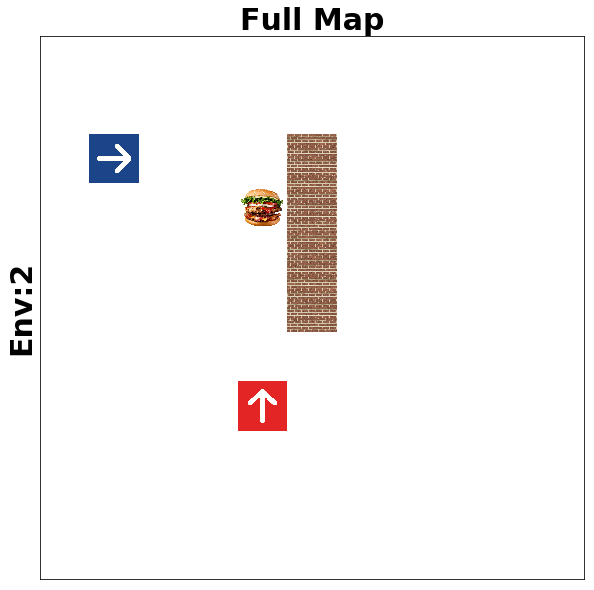
\includegraphics[scale=0.20]{figures/ENV:2_FM.png}}
\subfloat[]{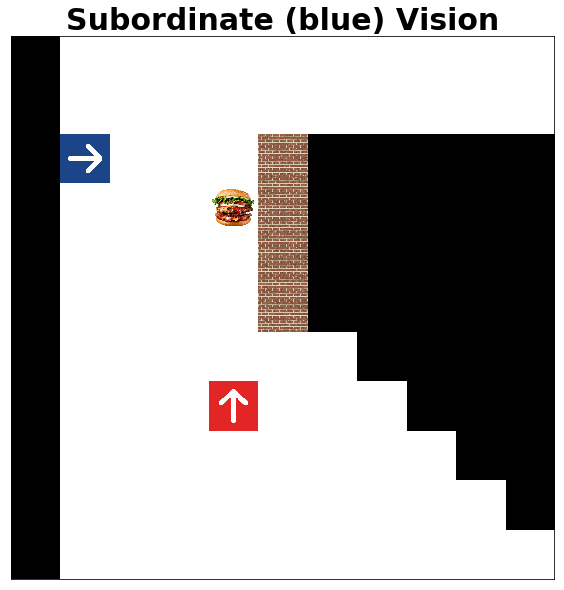
\includegraphics[scale=0.20]{figures/ENV:2_AI.png}}
\subfloat[]{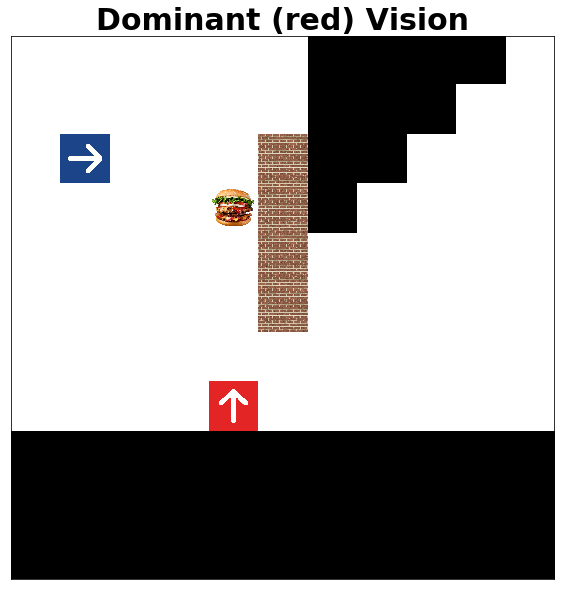
\includegraphics[scale=0.20]{figures/ENV:2_DM.png}}
    \caption{Test  case 2: \(A_{sub}\) avoided the food although the food is in the same position as in \texttt{Test case 1}. The only difference is the dominant position and direction: the dominant can see the food. The observed behavior is also what one would expect from an agent with the perspective taking ability.}
    \label{fig.tc.2}
\end{center}
\end{figure}
\begin{figure}[H]
\begin{center}
\subfloat[]{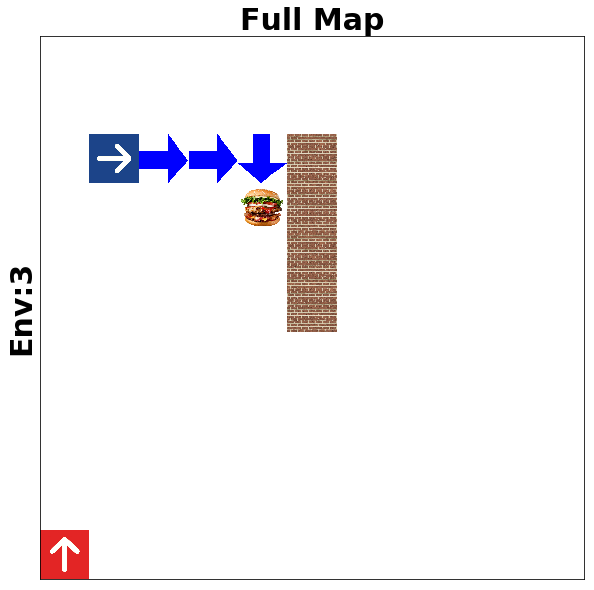
\includegraphics[scale=0.20]{figures/ENV:3_FM.png}}
\subfloat[]{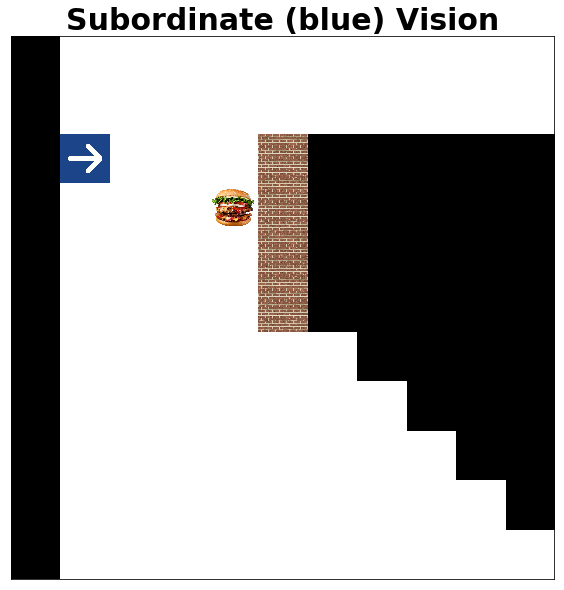
\includegraphics[scale=0.20]{figures/ENV:3_AI.png}}
\subfloat[]{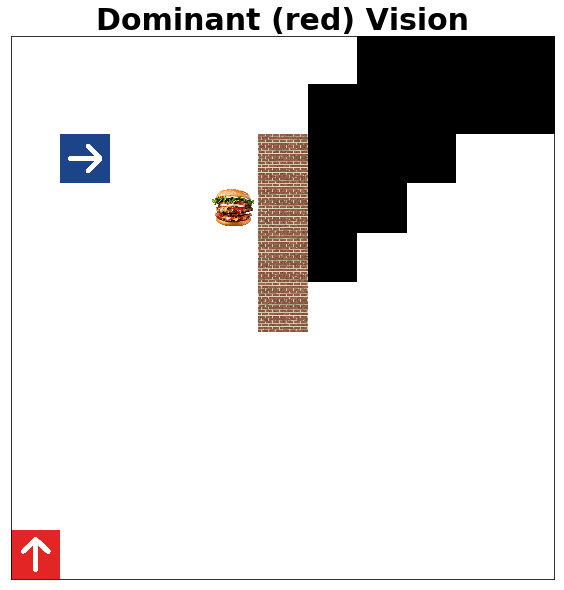
\includegraphics[scale=0.20]{figures/ENV:3_DM.png}}
\caption{Test  case 3: \(A_{sub}\) went for the food, although the dominant is there and able to see everything. However, the dominant was out of the field of vision of the subordinate and hence the subordinate never witnessed \(A_{dom}\) until the very last move of eating the food. This behavior is also expected to happen.}
\label{fig.tc.3}
\end{center}
\end{figure}
\begin{figure}[H]
\begin{center}
\subfloat[]{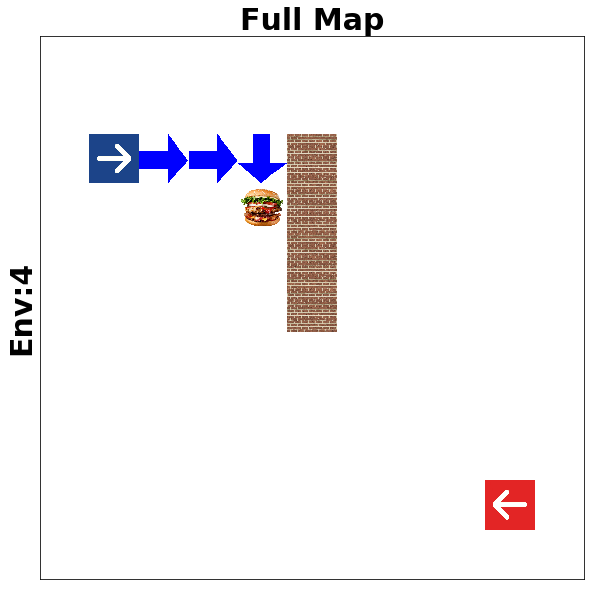
\includegraphics[scale=0.20]{figures/ENV:4_FM.png}}
\subfloat[]{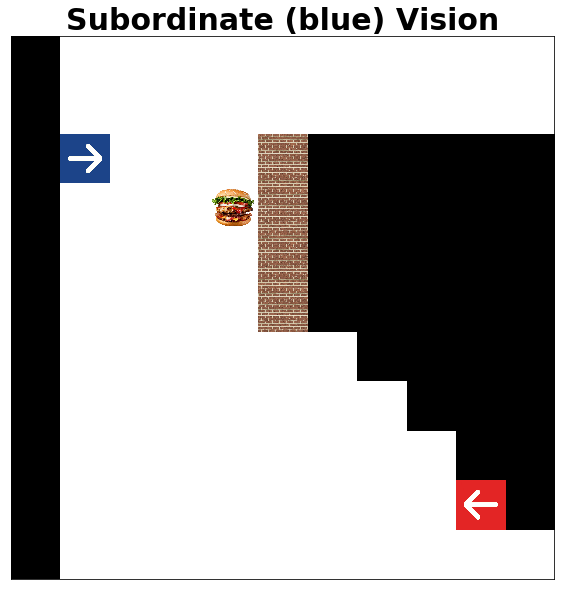
\includegraphics[scale=0.20]{figures/ENV:4_AI.png}}
\subfloat[]{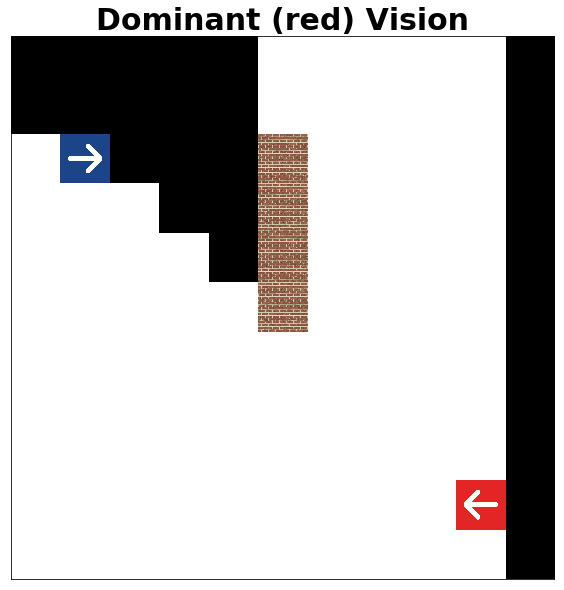
\includegraphics[scale=0.20]{figures/ENV:4_DM.png}}
\caption{Test  case 4: in this case the subordinate reached for the food. Although the dominant was looking toward the subordinate, the food was not visible for the dominant. This behavior matches what an agent with perspective taking would do.}
\label{fig.tc.4}
\end{center}
\end{figure}
\begin{figure}[H]
\begin{center}
\subfloat[]{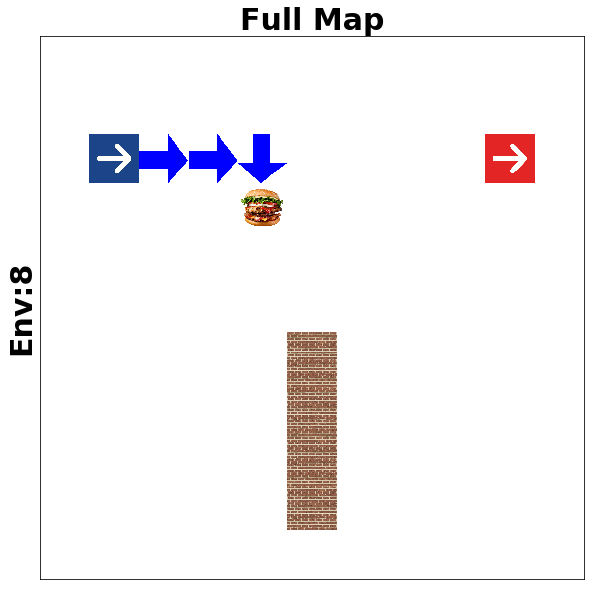
\includegraphics[scale=0.20]{figures/ENV:8_FM.png}}
\subfloat[]{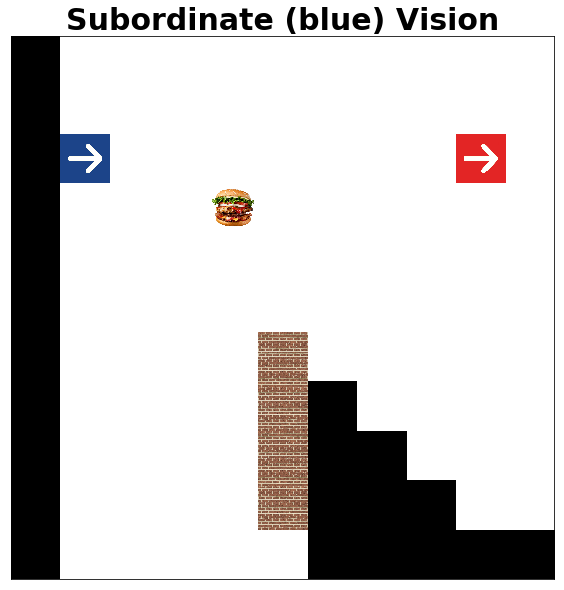
\includegraphics[scale=0.20]{figures/ENV:8_AI.png}}
\subfloat[]{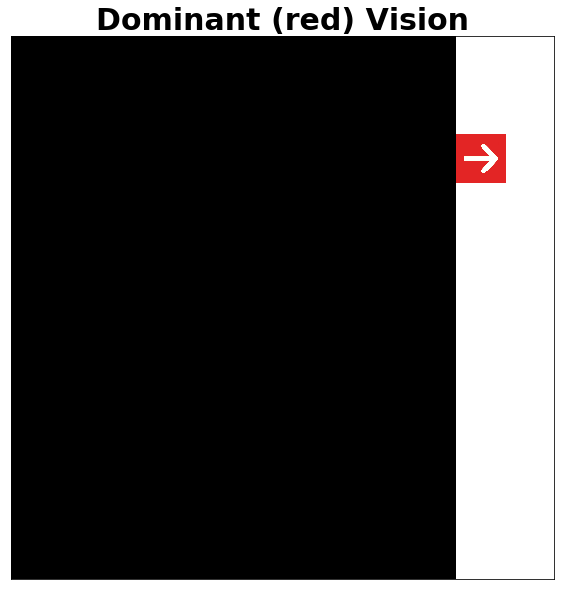
\includegraphics[scale=0.20]{figures/ENV:8_DM.png}}
\caption{Test  case 8: this test case is identical to test case 4 with the change in the distance between the dominant and the food. Although the dominant is closer to the food, it still cannot see it. The subordinate went for the food in this experiment which is a behavior to expect from an agent capable of perspective taking ability.}
\label{fig.tc.4}
\end{center}
\end{figure}
\begin{figure}[H]
\begin{center}
\subfloat[]{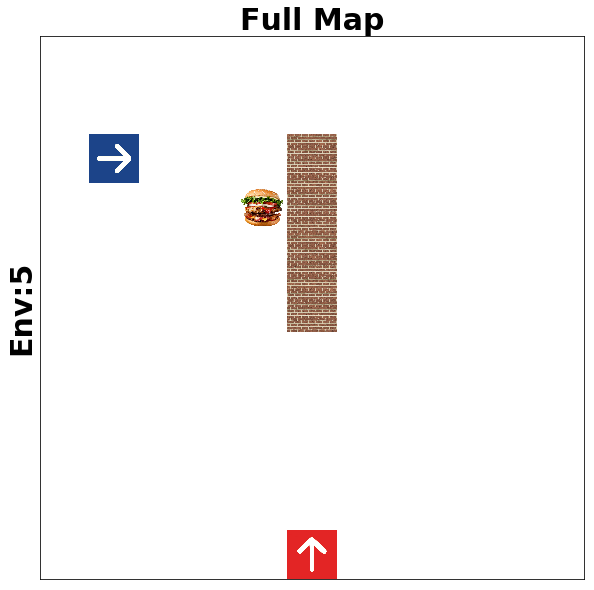
\includegraphics[scale=0.20]{figures/ENV:5_FM.png}}
\subfloat[]{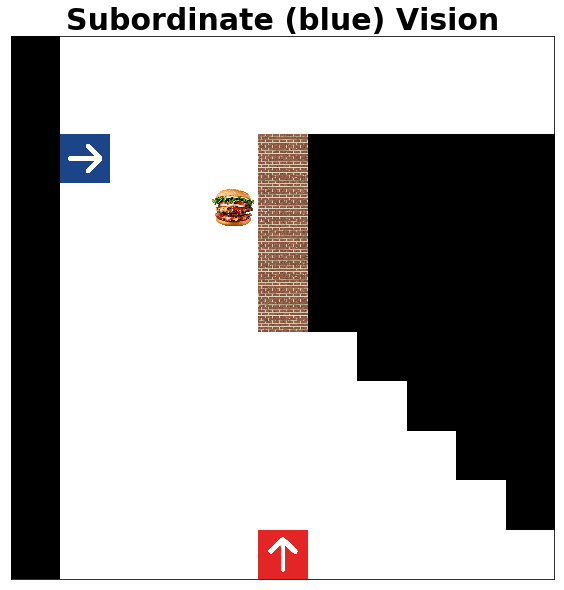
\includegraphics[scale=0.20]{figures/ENV:5_AI.png}}
\subfloat[]{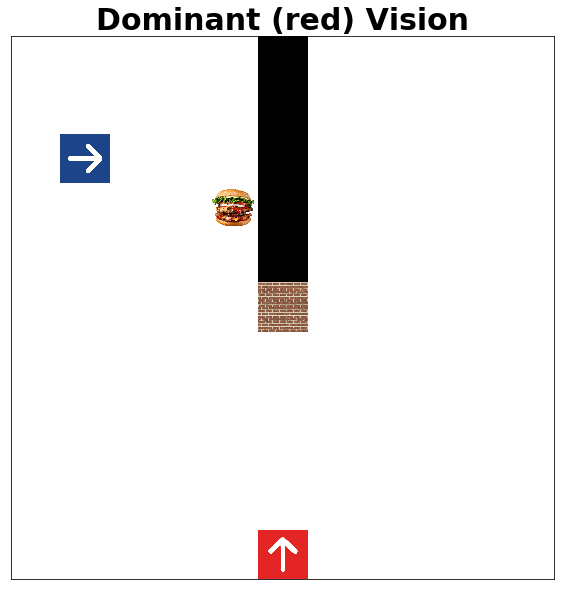
\includegraphics[scale=0.20]{figures/ENV:5_DM.png}}
\caption{Caption}
\label{fig.tc.5}
\end{center}
\end{figure}
\begin{figure}[H]
\begin{center}
\subfloat[]{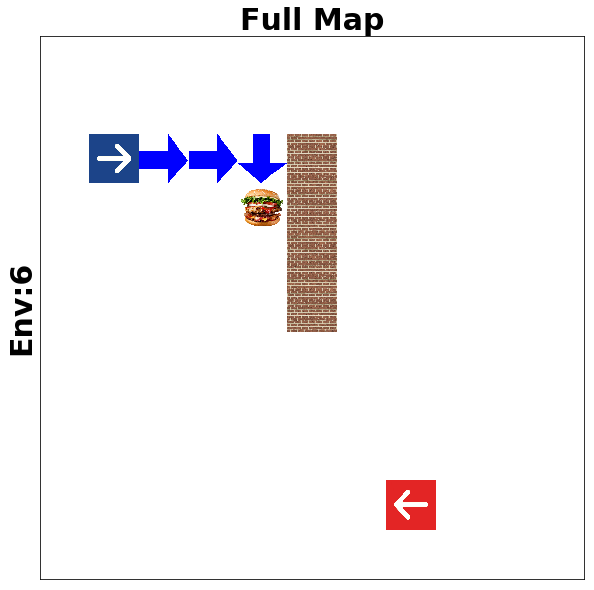
\includegraphics[scale=0.20]{figures/ENV:6_FM.png}}
\subfloat[]{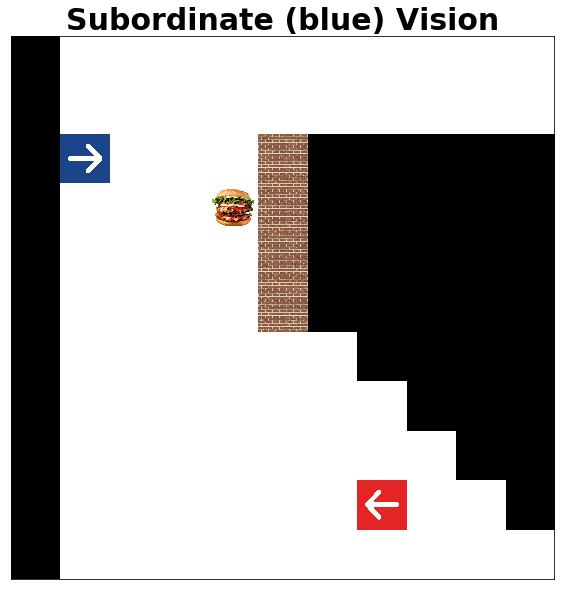
\includegraphics[scale=0.20]{figures/ENV:6_AI.png}}
\subfloat[]{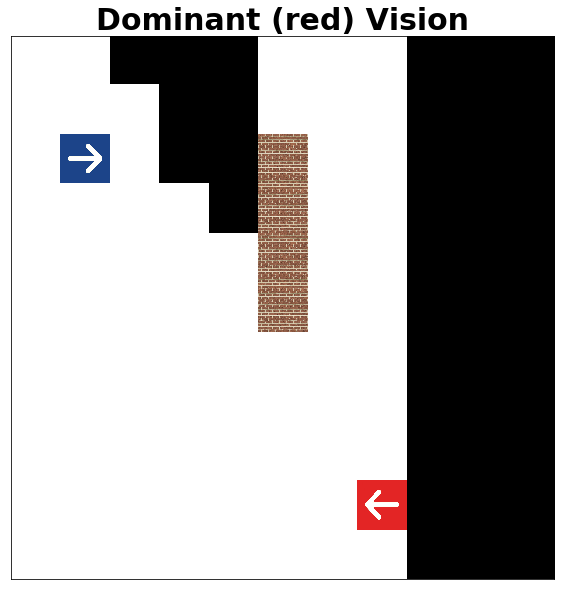
\includegraphics[scale=0.20]{figures/ENV:6_DM.png}}
\caption{\textbf {Test  case 6:} \(A_{sub}\) avoided the food although the dominant was not spotted in its field of view. It might be the case that food position is dangerous from previous experience while training. The same loopy behavior from previous test case is also spotted here.}
\label{fig.tc.6}
\end{center}
\end{figure}
\begin{figure}[H]
\begin{center}
\subfloat[]{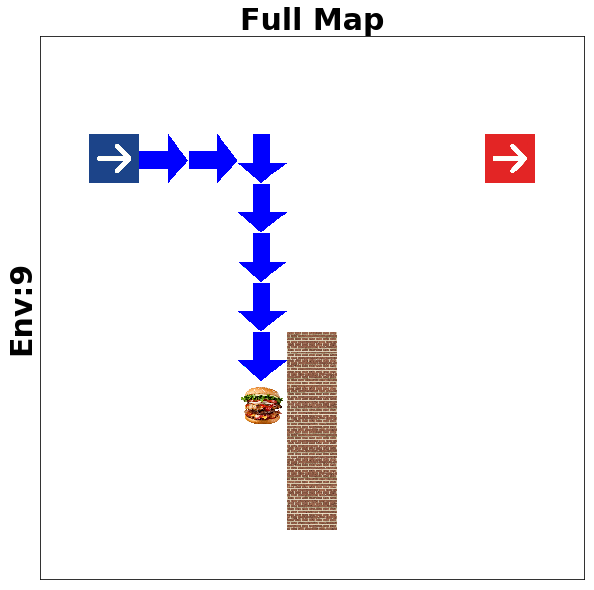
\includegraphics[scale=0.20]{figures/ENV:9_FM.png}}
\subfloat[]{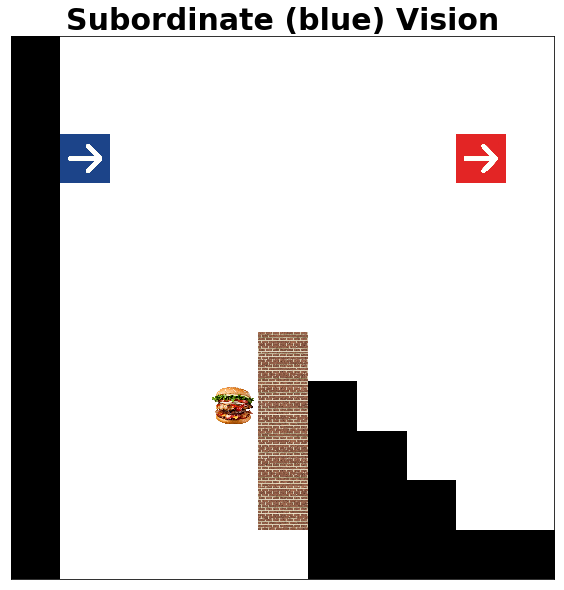
\includegraphics[scale=0.20]{figures/ENV:9_AI.png}}
\subfloat[]{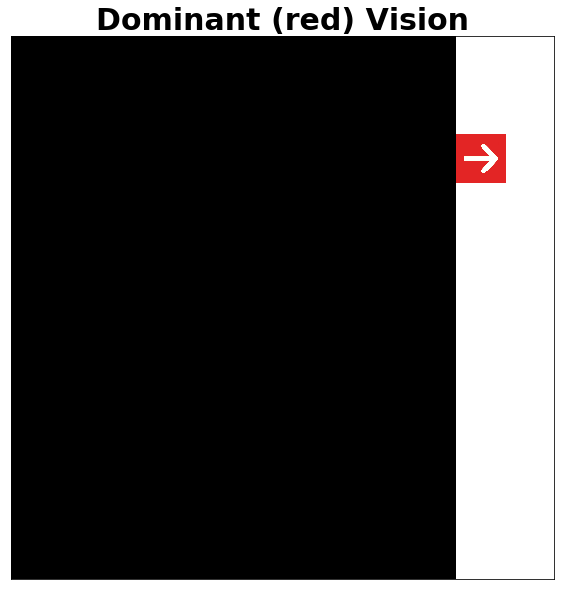
\includegraphics[scale=0.20]{figures/ENV:9_DM.png}}
\caption{Test  case 9: subordinate went for the food in this test case. Since the dominant was looking in the other direction, the food was not spotted by the dominant. Hence it is plausible to go for the food.  }
\label{fig.tc.9}
\end{center}
\end{figure}
\begin{figure}[H]
\begin{center}
\subfloat[]{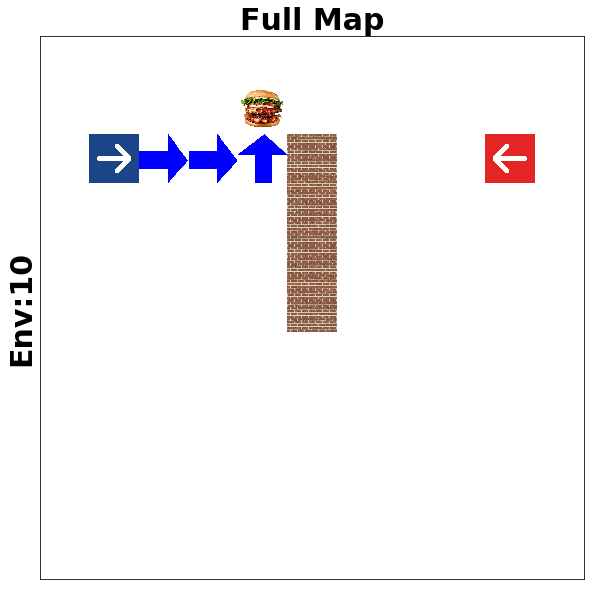
\includegraphics[scale=0.20]{figures/ENV:10_FM.png}}
\subfloat[]{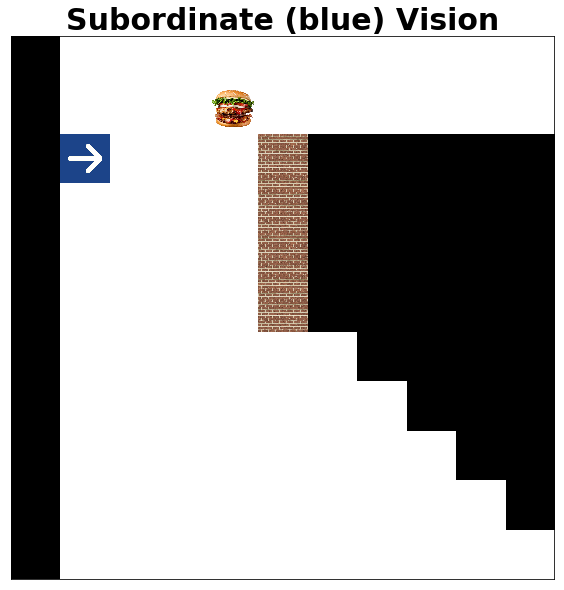
\includegraphics[scale=0.20]{figures/ENV:10_AI.png}}
\subfloat[]{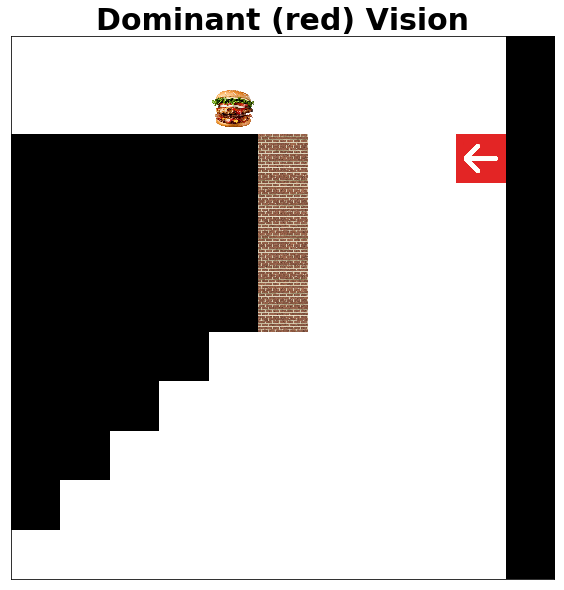
\includegraphics[scale=0.20]{figures/ENV:10_DM.png}}\\
\caption{Test  case 10: in this case we changed the food place and the obstacle where they are not seen by dominant. The subordinate retrieved the food successfully which is a behavior coincide with perspective knowledge.} 
\label{fig.tc.10}
\end{center}
\end{figure}
\begin{figure}[H]
\begin{center}
\subfloat[]{\includegraphics[scale=0.20]{figures/ENV:16_FM.png}}
\subfloat[]{\includegraphics[scale=0.20]{figures/ENV:16_AI.png}}
\subfloat[]{\includegraphics[scale=0.20]{figures/ENV:16_DM.png}}
\label{fig.tc.16}
\caption{TTest  case 16: \(A_{sub}\) go for the food. In this test case \(A_{sub}\) should or should not go to the food based on the trajectory followed. As we can see in Figure (\ref{fig.10}) \(A_{dom}\) was never spotten by \(A_{sub}\).} 
\end{center}
\end{figure}
\subsection{Most effective neurons}
To open the network we decided to check the most important neurons which basically hold highest weights. We took the neurons with highest weights that is connected to state value. Afterward we tried to see what those neurons represent, what areas they focus on and how much the dominant agent orientation important. To see these information we draw the weights between the inputs and those two neurons. \ref{fig.PN_61},\ref{fig.SN_61} show the neuron with highest positive weight and Figure \ref{fig.PN_76},\ref{fig.SN_76} show the neuron with highest negative weight. Those two neurons might be explained as desire for food and fear from dominant. 
\begin{figure}[H]
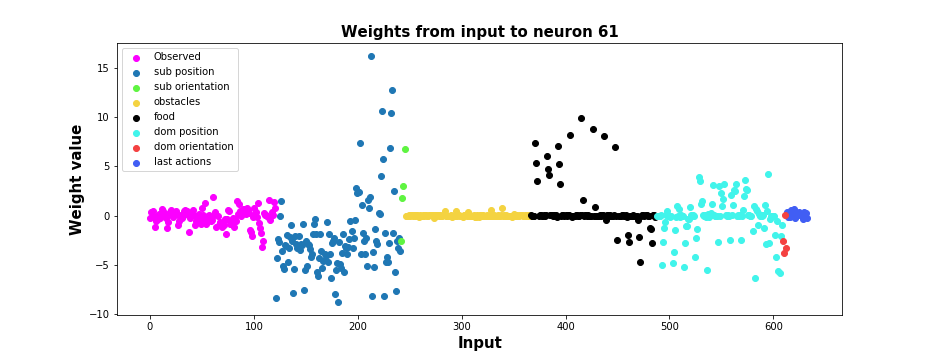
\includegraphics[scale=0.5,trim={3.5cm 0cm 2cm 0.5cm},clip]{figures/PN_61.png}
\caption{each color represent one group of input. The higher the value, the more weight is assigned to that specific input. A biological representation of this neuron might be the agent desire for food.weights over the input for most positive neuron.}
\label{fig.PN_61}
\end{figure}
\begin{figure}[H]
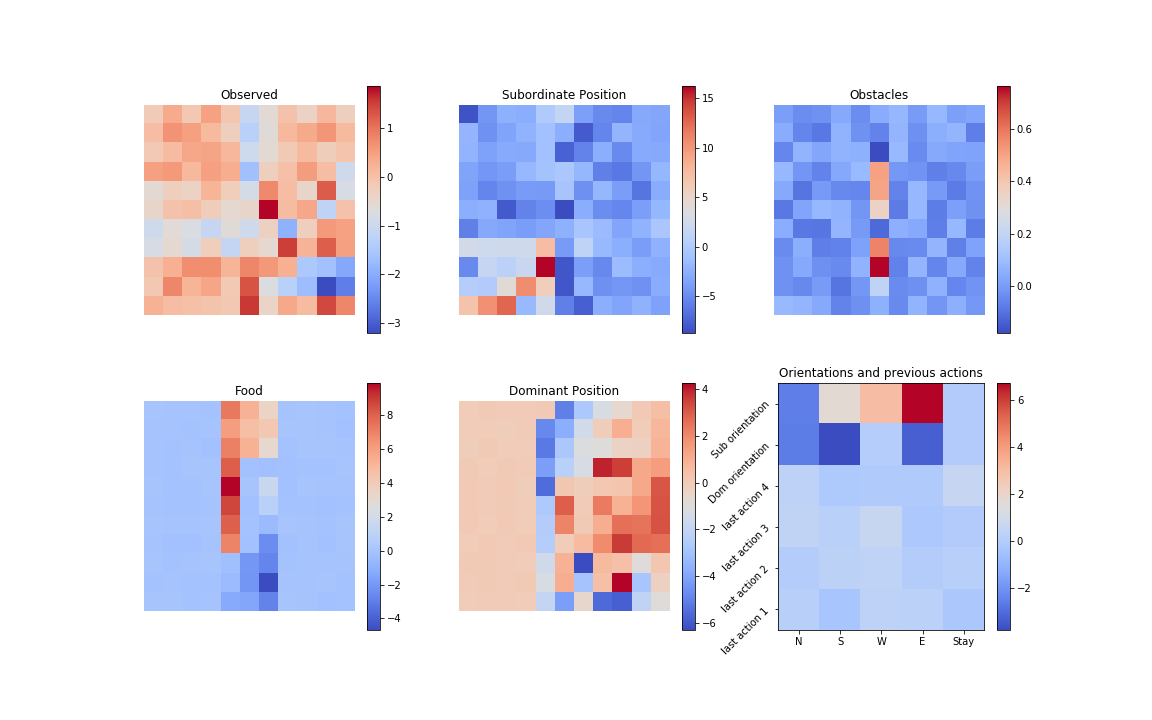
\includegraphics[scale=0.5,trim={5cm 2cm 4cm 3cm},clip]{figures/SN_61.png}
\caption{The weights between the input and hidden layer for neuron 61. We can see network weights mapped on environment for neuron with most
positive weights.}
\label{fig.SN_61}
\end{figure}
\begin{figure}[H]
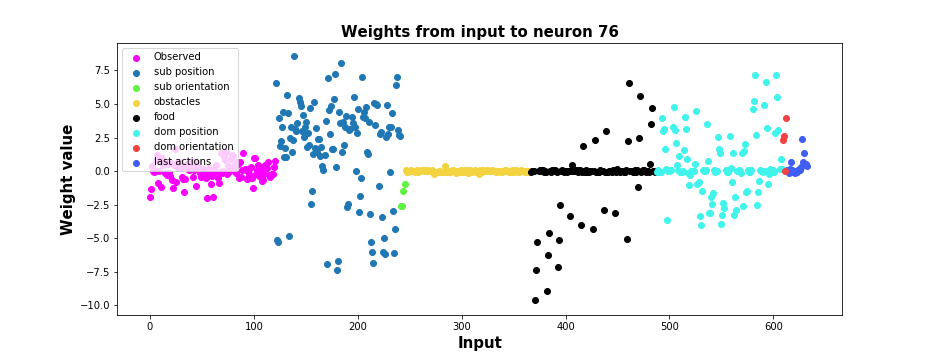
\includegraphics[scale=0.5,trim={3.5cm 0cm 2cm 0.5cm},clip]{figures/PN_76.png}
\caption{weights over the input for most negative neuron.}
\label{fig.PN_76}
\end{figure}
\begin{figure}[H]
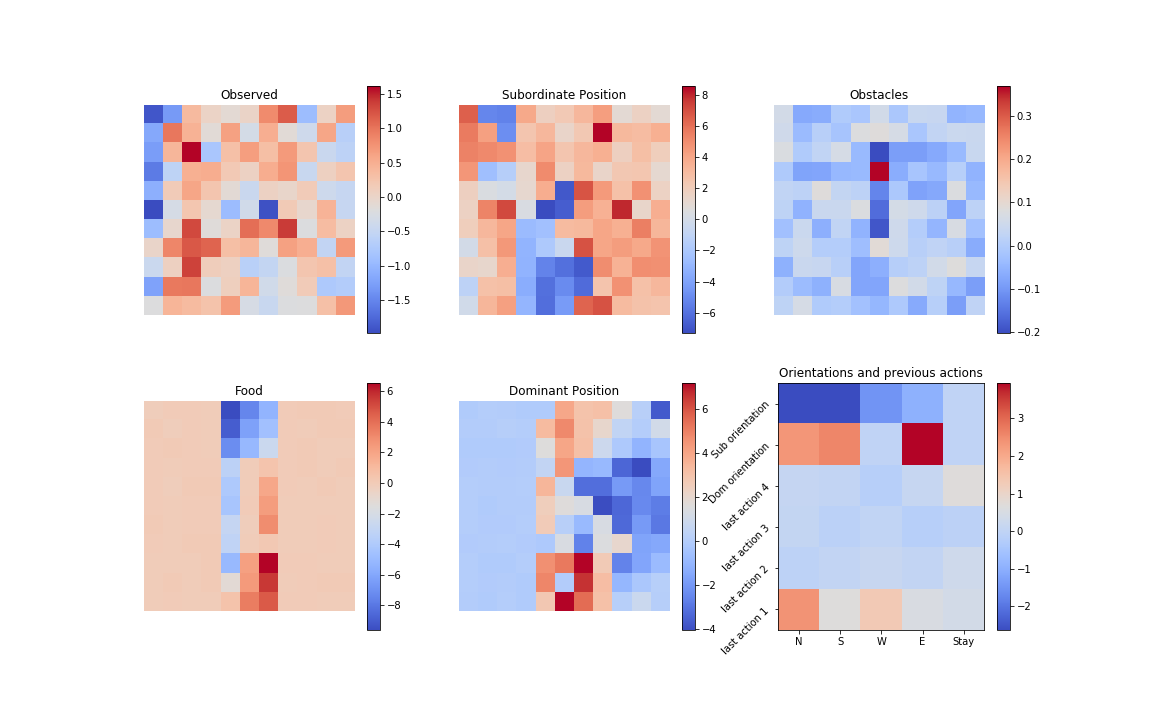
\includegraphics[scale=0.5,trim={5cm 2cm 4cm 3cm},clip]{figures/SN_76.png}
\caption{network weights mapped on environment for neuron with most negative weights.}
\label{fig.SN_76}
\end{figure}
We recorded the hidden nodes values over those 10 cases with there variations. Afterward we applied T-SNE to draw the points in 2d. We can clearly see from Figure \ref{fig.expected.behavior}

\begin{figure}[H]
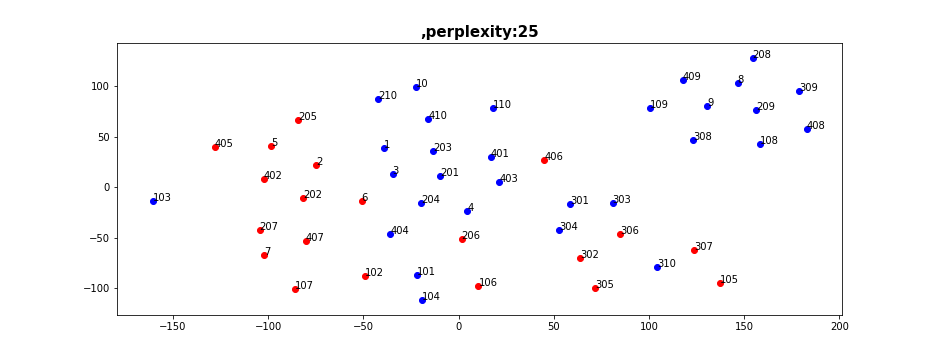
\includegraphics[scale=0.5,,trim={3.5cm , 1.5cm , 0cm , 0cm},clip]{figures/EB.png}
\caption{T-SNE over the activations over initial states for all 50 test cases. Blue: expected behavior is to go toward food, while red expected not to go toward food.}
\label{fig.expected.behavior}
\end{figure}
\begin{figure}[H]
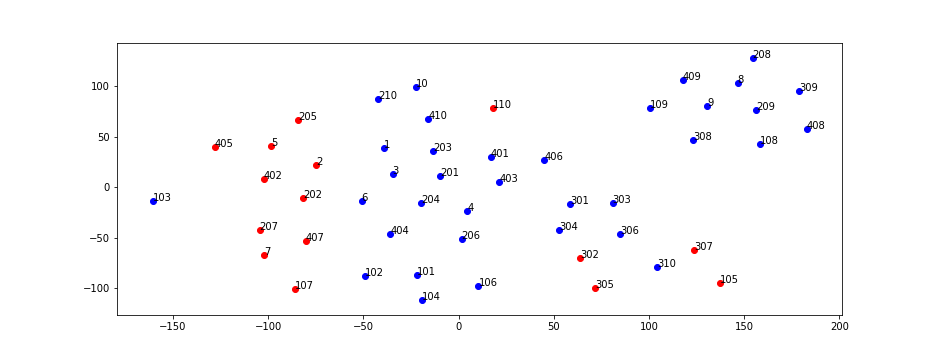
\includegraphics[scale=0.5,trim={3.5cm , 1.5cm , 0cm , 0cm},clip]{figures/AB.png}
\caption{T-SNE over the activations over initial states for all 50 test cases. Blue: went  to food, while red did not.}
\label{fig.actual.behavior}
\end{figure}

\section{Conclusion}
In this paper we showed 10 test cases that require perspective taking to be accomplished. Those test cases and their variations were solved by an artificial neural network trained with RL. The behavior of the agent showed evidence for basic perspective taking skills. By changing only the position of the dominant while keeping the positions of the subordinate, the food and the obstacle the same, we observed that the subordinate either went for the food or not depending on the position of the dominant (compare test cases 1xxx and 2xxx figure xxx). Even when the dominant was in the field of view of the subordinate, the subordinate went for the food if the dominant could not see the food (test case 4xxx, Figure xx).  

We also presented a detailed analysis of the weights of the hidden layer and the activation over all the test cases with T-SNE. All T-SNE figures concluded to two clusters which make us believe that the network could be simplified even more. 

In the present work with relatively simple deep RL agents we observed that the subordinate agent can learn to take into account the behavior of the dominant agent through trial-and-error over a long training period. This is in stark contrast to chimpanzees who master the particular task in the first trial  (Hare et al 2000; 2001). However, it is important to note that the chimpanzees had learned about social hierarchies and about the behavior of other chimpanzees in their daily life over many years. Hence, the fact that in the present work the subordinate agents learned to take into account the behavior of the dominant agent demonstrates that at least part of perspective taking skills can indeed be learned through reinforcement learning. 

We are not claiming that RL would capture all aspects of mindreading. We simply feel that by understanding the capabilities and limitations of RL agents in acquiring mindreading we will better understand the computational demands of mindreading, just as deep neural networks have led to a better understanding of vision.


The results we have push us toward that the needed ingredients for perspective taking might be much less than what we think is needed. It might be the position of the elements and orientation sufficient enough for perspective taking to emerge without the need for imagining what the dominant can or can not see. Further research still needed with simpler or more complex architecture. Although the current simple network did the job, there are probably other networks with interesting interpretation. Our next step is to add more architectural changes to the network. To be exact adding memory to the network to make it one step closer to brain.
\bibliographystyle{plain}
\bibliography{references}
\appendix
\section{\\Test cases}\label{test.cases}
% the \\ insures the section title is centered below the phrase: AppendixA

\section{Title of Appendix B}
% the \\ insures the section title is centered below the phrase: Appendix B

Text of Appendix B is Here
\end{document}
